\newpage
\section{Procedimento Experimental}

\subsection{Materiais Utilizados}

\subsubsection{Materiais de Laboratório}
Os materiais utilizados em bancada foram:

\begin{itemize}
	\item Conectores de cobre;
	\item Resistor de $1 k\Omega$;
	\item Capacitor de $1 \mu F$;
	\item indutor de $10 mH$
	\item Módulo PU-2222;
	\item Protoboard;
	\item Gerador de função;
	\item Conectores “Banana-jacaré”;
	\item Osciloscópio digital;

\end{itemize}

\subsubsection{Softwares de Simulação}
O software utilizado para simulação do circuito foi o Multisim Live \cite{multisim}, um software de simulação de circuitos gratuito e eficiente perante os objetivos do experimento.

\subsection{Metodologia}
À priori, o circuito foi analisado diante dos seguintes aspectos: Função de transferência, o módulo da função de transferência, para $\omega=0$, $\omega\rightarrow\infty$ e $\omega=\omega_n$, tanto considerando a tensão de saída como a tensão sobre o resistor (filtro rejeita-faixa), quanto a tensão sobre o paralelo LC (filtro passa-faixa).

É importante ressaltar que neste experimento, o filtro passa-faixa e filtro rejeita-faixa são analisados no mesmo circuito, portanto, o mesmo deve ser montado (vide Figura \ref{circuitoSimulado}, e assim é possível analisar ambos os comportamentos simultaneamente. Veremos com mais detalhes a seguir.

É necessário que, além do circuito apresentado no roteiro (Figura \ref{circuitoRoteiro}), sejam incluídos o terra e os voltímetros. Com os voltímetros localizados nestes pontos, é possível analisar a tensão nas extremidades do resistor com PR2 e no paralelo entre o indutor e o capacitor, com PR1. Com isso, a frequência deve ser alterada manualmente perante os valores de $\omega_{C1}$, $\omega_{C2}$ e $\omega_0$ calculados teóricamente, com o objetivo de observar e analisar as respostas gráficas do circuito. Além das frequências em questão, as respostas também devem ser analisadas para os valores presentes na tabela disponibilizada no roteiro, de modo que as lacunas possam ser preenchidas.

\begin{figure}[H]
	\centering
	\caption{Diagrama do Circuito RLC.}
	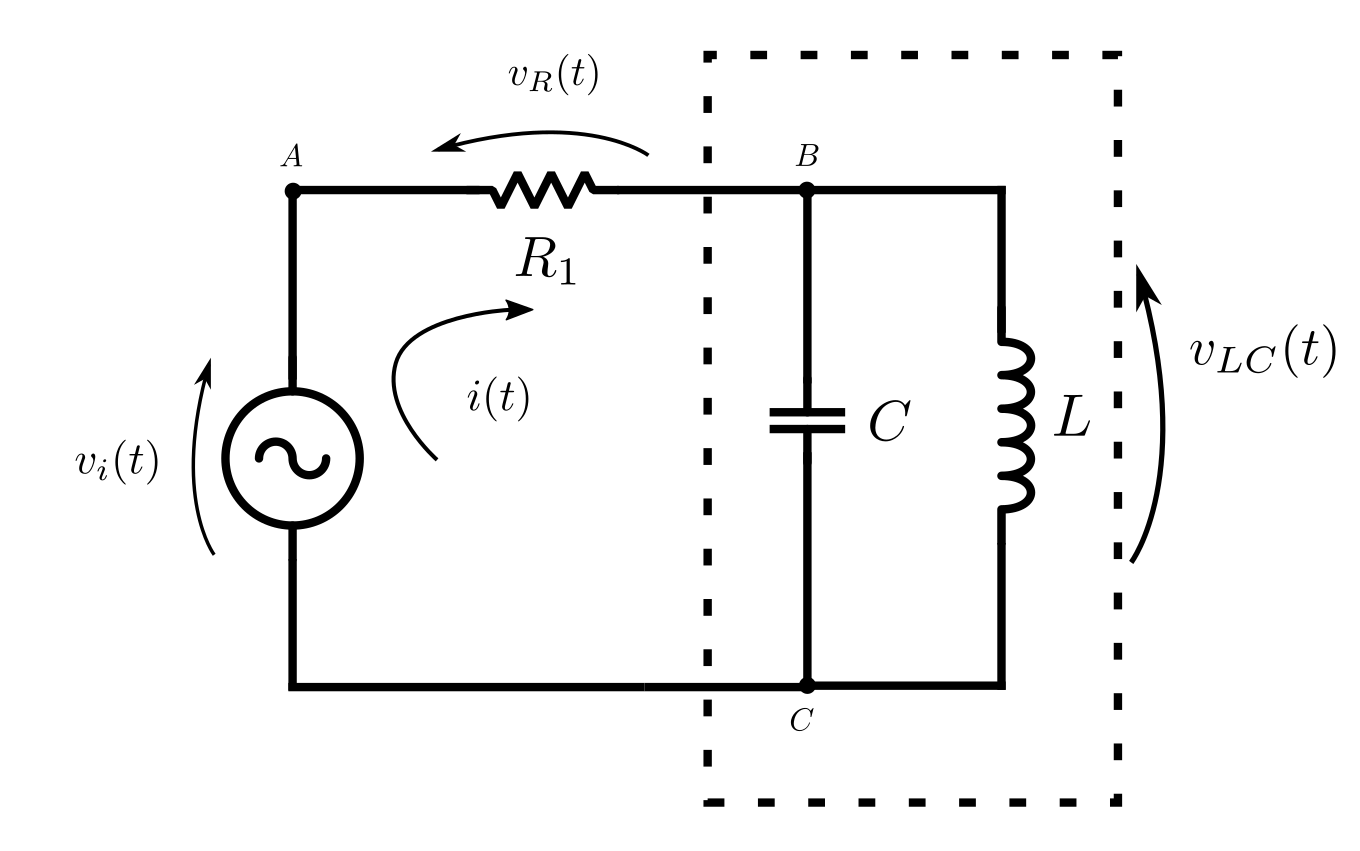
\includegraphics[width=15cm]{imagens/circuitoRoteiro.png}
	\caption*{Fonte: \cite{roteiro4}.}
	\label{circuitoRoteiro}
\end{figure}

\pagebreak